
\subsection{Verdande models} \label{Section:VerdandeModels}

As has been pointed out in Deliverable D1.2 \cite{Fer14b}, three main tasks have to be addressed for Verdande Technology use case:

\begin{enumerate}
\item \textbf{Automatic detection of drill string vibrations and abnormal torque states}: which aims to better diagnose the shape of the wellbore and the state of the equipment, make better decisions on how to manage the well, and thereby reduce the non-productive time. To this end, a probabilistic graphical model for erratic torque monitoring and detection will be used.

\item \textbf{Semi-automatic labelling}: Given unlabelled data streams collected over time from typical drilling conditions, semi-automatic labelling aims to compute a normality score for each considered drilling situation, then label it as either ``normal'' or ``abnormal''. As for the previous task, a probabilistic graphical model will be used, taking into account the temporal dynamics of the drilling process and continuously adapting to changes in the incoming streaming data. 

\item \textbf{Automatic formation detection}: which aims to predict in real time the formation tops from the MWD (measurements while drilling) data using a probabilistic graphical model. Once again, this should be performed taking the temporal dynamics of the drilling process into account. The automatic formation detection is vital for dealing with several issues such as hole instability and vibrations, and also important for reducing the costs and the overall non-productive time.
\end{enumerate}

%For all tasks, the model must deal with both continuous and discrete random variables. Moreover, the oil-well data to be used has the following characteristics: 
%
%\begin{itemize}
%
%\item It has a dynamic structure consisting of \emph{long-term} patches (ranging from a couple of hundred observations and into the thousands). Inside a patch, the data is typically fairly \emph{stable} and with low noise, even if this is not always the case. Between the patches the data can vary a lot. A \emph{patch of data} typically corresponds to the implementation of one activity (like drilling, connection tripping in/out, etc.). Consequently, models may potentially be designed to operate locally inside a single patch.
%
%\item Inside one activity, many of the attributes can be strongly correlated. The observed correlation between variables $X$ and $Y$ can either be instantaneous (i.e., corr($X_t, Y_t$) is significant), or delayed to some extent (i.e., exposed through the correlation corr($X_t, Y_{t+v}$) for some fixed lag $v$).
%
%\item Physical models can to some extent be used to understand why the correlations are present, but not to quantify them. In addition, sometimes the strength, and even the sign, of the correlation may change from well to well.
%
%\end{itemize}

The following 3 subsections detail the designed models for the different use cases.

%-------------------------------------------------------------------------------------------------------------------------------------------------------------------
\subsubsection{Detection of drill string vibrations and abnormal torque states}\label{SubSection:DetectionTorque}
%-------------------------------------------------------------------------------------------------------------------------------------------------------------------

The hole drill string, including the bottom hole assembly and the bit, is designed to transfer as much energy as possible from the rotary table to break rock at the bit.  When this energy transfer is inefficient, the energy goes into shaking the drill string.  This involves drilling slower, a higher risk to break equipment and a lower hole quality. Automatic detection of drill string vibrations can help the drilling crew to better diagnose both the condition of the equipments and also the hole itself. Drillstring vibrations are seen as an erratic torque signal on the realtime data.  We have therefore focused on detection of erratic torque.

Two time-windows of torque-readings are given in Figure \ref{Figure:VTTorqueValues}; the uppermost plot traces the torque over a period of 25.000 observations, the other is zoomed in to cover only 500 observations. It is evident that the torque varies over time, and often drops to zero (in particular when the drill-bit is not rotating). Furthermore, we can see from the zoomed-in trace that the variance changes over time; this time-window commences with rapidly varying torque, before the variation is reduced. The goal is to extract passages where high variance in the observed torque cannot be explained by other drilling parameters. 
We will begin the following discussion by considering how to model the torque as a random variable developing over time, without thinking about vibration and the variable's relationship to other drilling parameters. Thereafter, a full model will be proposed.

\begin{figure}[ht!]
\begin{center}
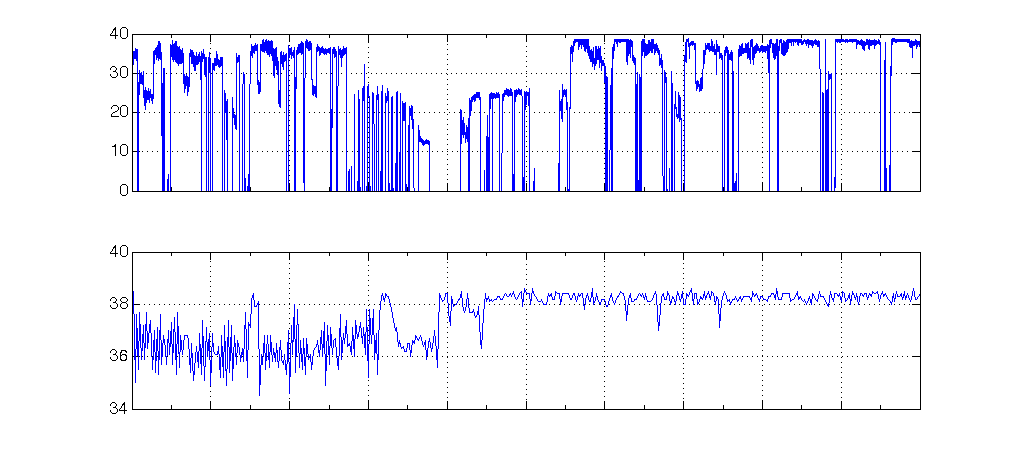
\includegraphics[scale=0.3]{./figures/VT_TRQ_values} 
\caption{\label{Figure:VTTorqueValues} Measurements of the torque over two time-windows.}
\end{center}
\end{figure}

The sample correlogram and sample partial correlogram of the torque can be seen in Figure \ref{Figure:VTTorqueAutoCorr}. Note that only the data from drilling (i.e., where the torque is positive and ``moving naturally'') have been included in these calculations. It is clear that a significant autocorrelation exists, also at high lags. The figure goes up to lag $v=20$, where the correlation is still above $0.6$. Furthermore, the partial correlogram shows very significant contributions at lags 1 and 2, and also significant effects at lags 5 --10. A model capturing the time dynamic is therefore essential. 

\begin{figure}[ht!]
\begin{center}
\begin{tabular}{c@{}c}
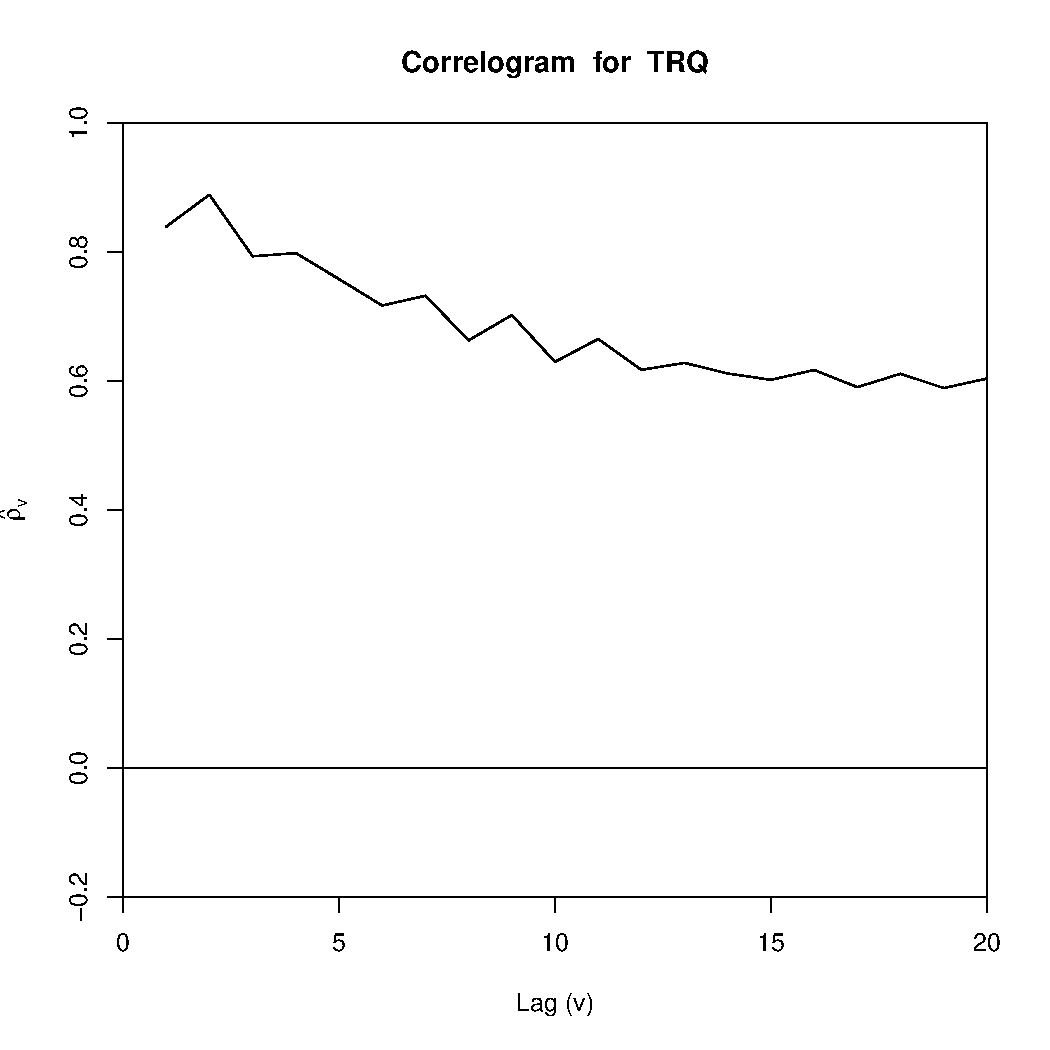
\includegraphics[scale=0.4]{./figures/Verdande_Corr_TRQ.pdf} &
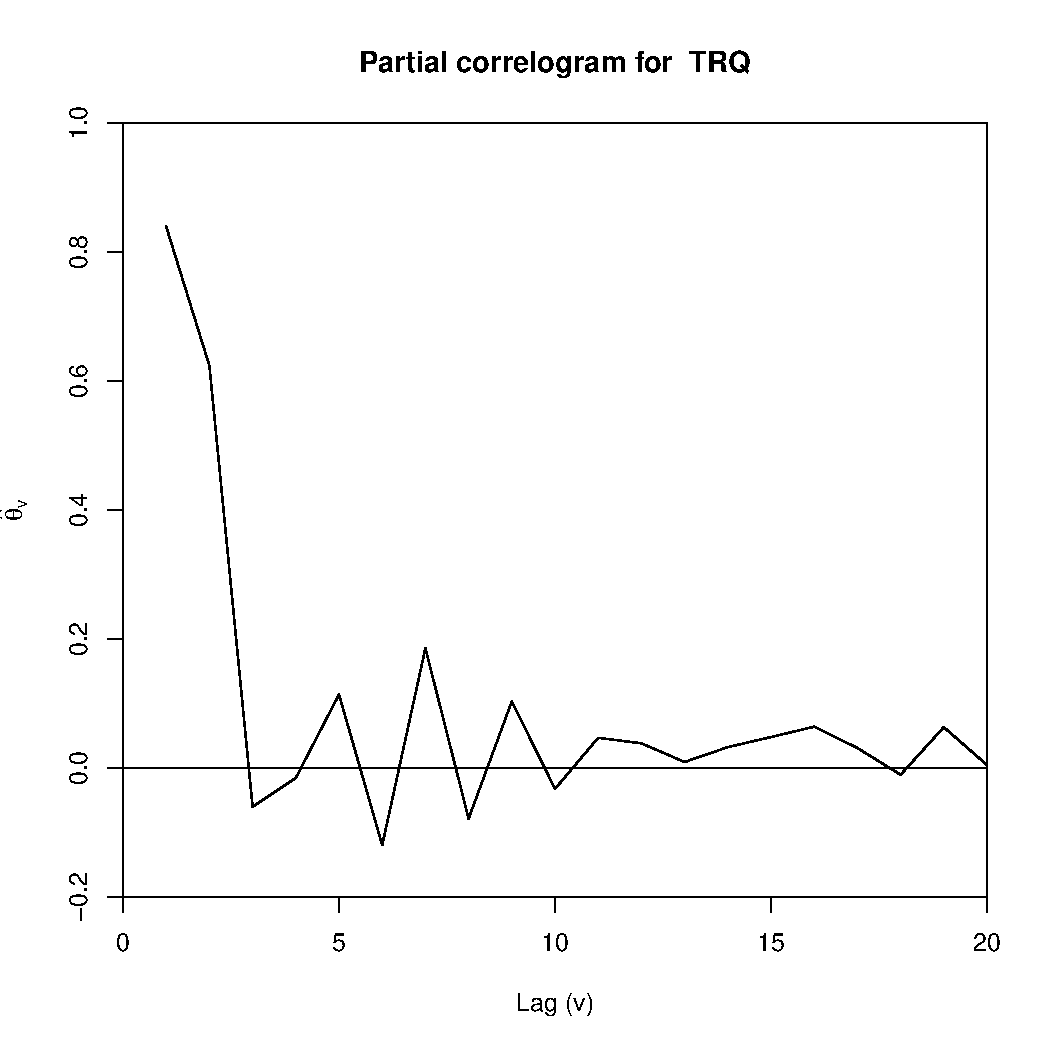
\includegraphics[scale=0.4]{./figures/Verdande_ParCorr_TRQ.pdf}  \\
\end{tabular}
\caption{\label{Figure:VTTorqueAutoCorr} Correlogram and partial correlogram of the torque while drilling.}
\end{center}
\end{figure}

To capture the dynamics of the torque variable, we propose a KF model (see \ref{SubSubSection:KFs}), with a sufficiently ``rich'' latent variable space (that is, more than a single one-dimensional latent variable may be required to capture the partial autocorrelations in the data). 

Next, we consider how to model a torque sequence that also includes abnormal torque measurements (those that are corrupted by vibrations). Our working assumption is that an abnormal torque signal is the result of a string vibration with frequency higher than the sampling frequency of the data. Thus, it will be observed as a white-noise signal superimposed on top of the ``true'' underlying torque signal. An abnormal torque regime will typically last for some unknown time significantly longer than one time step, thus we must create a model with the ability to choose a state that fits the observations best (normal or abnormal), and with a tendency to remain in a chosen state over time. This can be obtained by an SKF (see \ref{Figure:SKF}), where the switching variable (connected over time) is used to show which state one is in at a given time (normal or abnormal) and the transition model for the variable is used to capture the state remaining for some time. 

Preliminary results using this model class, but without learning the parameters properly, and relying on an inference scheme that does not scale to the data-sizes we have available in the AMIDST project, are shown in Figure \ref{Figure:VTEraticTorqueMarked}. The same 500 data points shown  in Figure \ref{Figure:VTTorqueValues} are once again used, and the positions the system detects as having ``abnormal torque'' are highlighted in red along the $x$-axis. These annotations correlate well with what can be obtained by simple inspection of the time series with the human eye. 

\begin{figure}[ht!]
\begin{center}
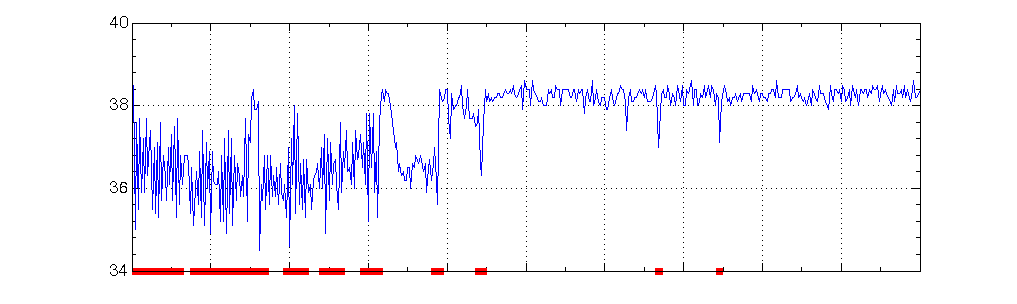
\includegraphics[scale=0.3]{./figures/VT_ErraticTRQ_marked} 
\caption{\label{Figure:VTEraticTorqueMarked} Values of torque in normal (blue line) and abnormal (red bottom marks) states resulting from an inference process performed on a SKF.}
\end{center}
\end{figure}

Still, some undesired annotations remain. For instance, the two areas with small dips in the observed torque towards the end of the sequence can be explained by specific drilling activities going on, and should not be marked as abnormal. To capture this, the context of the torque observation must be included, which is what we turn to next.

The parameters in drilling can to some extent be seen as control-response pairs. The control parameters are the flow, the rotation speed and the position of the brake handle under drilling. The position of the break handle is usually not recorded, but the response of all this is the hook load and thereby the weight on the bit (WOB), the pressure at the top of the drill string, the torque (TRQ) and the rate of penetration (ROP). In general, the control parameters are adjusted to increase ROP as much as possible. In particular, ROP and TRQ are correlated.

To analytically examine the relationship between ROP and TRQ further, we plot the joint density of (ROP$_t$, TRQ$_t$) and the sample correlogram between ROP$_t$ and TRQ$_{t+k}$ in Figure \ref{Figure:VTTorqueRateOfPenetration}. We notice that even if a strong correlation is not apparent in the density plot, it can be seen as significant from the correlogram. Hence, ROP could give some information about TRQ. Our intention here is to exploit this information to improve the accuracy of the detection of ``abnormal torque'' readings and avoid those false positives which appeared in Figure \ref{VT_ErraticTRQ_marked}. In terms of modelling, we update the initial SKF by introducing ROP as an ``input variable'' shown in  in Figure \ref{Figure:VTScenario1}, which results in a so-called \textit{input-output SKF} (IOSKF) model. 

\begin{figure}[ht!]
\begin{center}
\begin{tabular}{c@{}c}
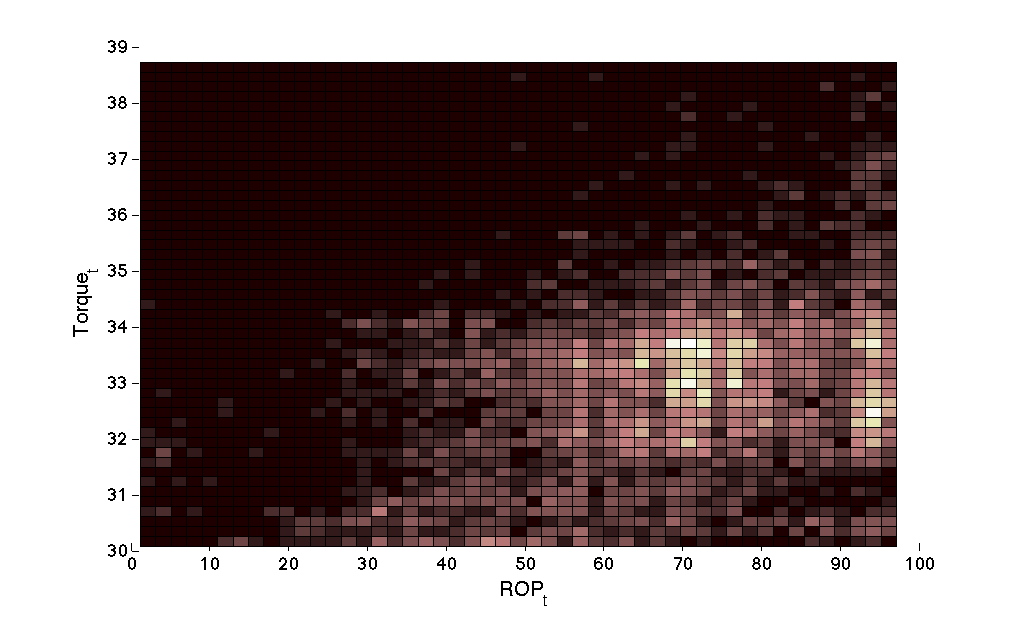
\includegraphics[scale=0.25]{./figures/VT_TRQ_ROP_density} &

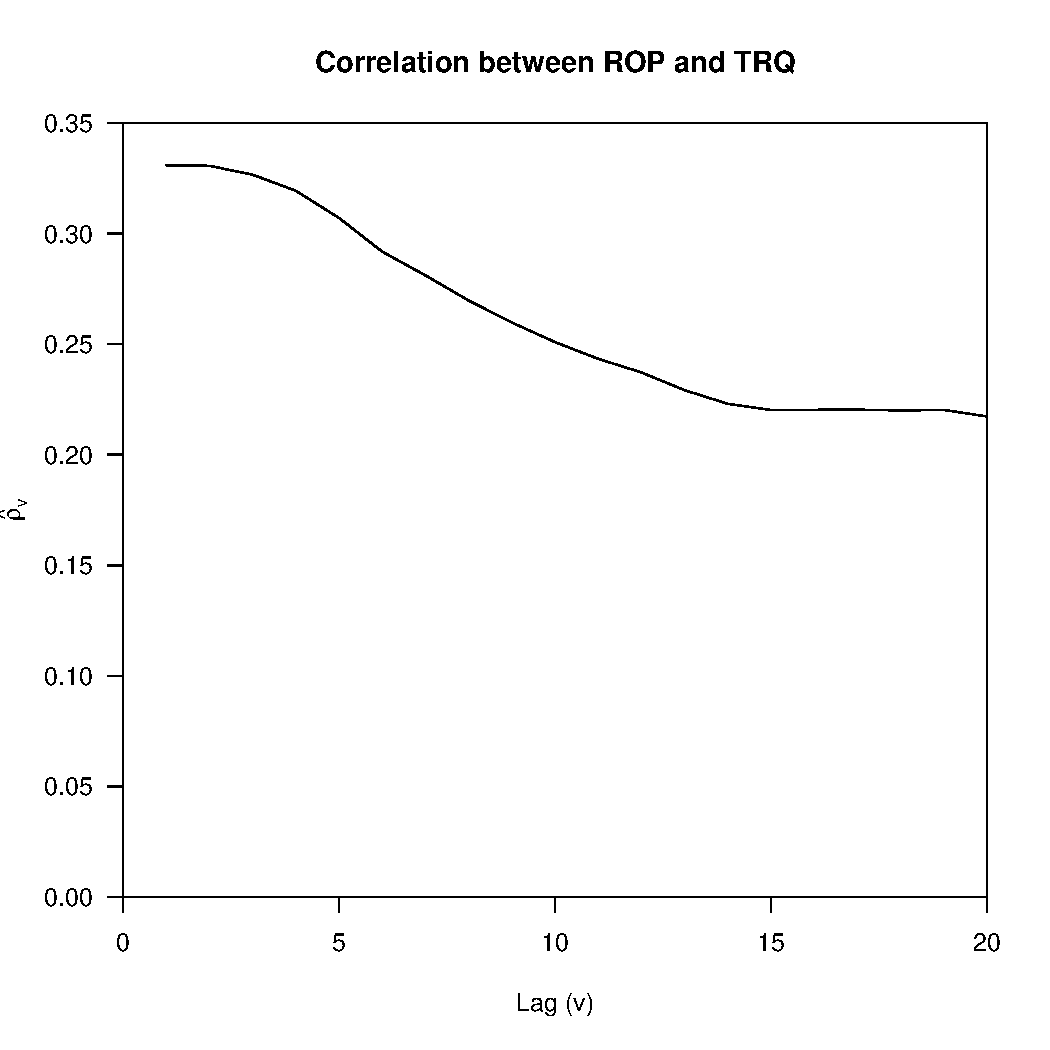
\includegraphics[scale=0.32]{./figures/Verdande_Corr_TRQ_vs_ROP.pdf}  \\
\end{tabular}
\caption{\label{Figure:VTTorqueRateOfPenetration} Left: joint density of (ROP$_t$, TRQ$_t$) and right: sample correlogram between ROP$_t$ and TRQ$_{t+k}$. }
\end{center}
\end{figure}

In the IOSKF model, the ``input'' at time $t$ is the ROP at that point in time, the ``output'' is the (observed) TRQ readings\footnote{It is generally the case that the output variables in the input-output dynamic models correspond to the target variables and are hence not observed during inference \cite{barberBRML2012}. In our case, however, the target variables correspond to a discrete state/hidden variable whereas the output variables will be observed during inference. See Section \ref{SubSubSection:HMMs} for further details.}, and we have two sets of latent variables: $i)$ a discrete switching variable, which is used to determine which TRQ regime we are currently in, and $ii)$ a latent vector of continuous variables used to capture and model the natural behaviour of the TRQ sequence over time. During inference, the posterior probability of the discrete latent variable at time $t$ can be used to detect whether or not the system experiences abnormal TRQ (that is, not explained by the observed ROP) over time. 

\begin{figure}[ht!]
\begin{center}
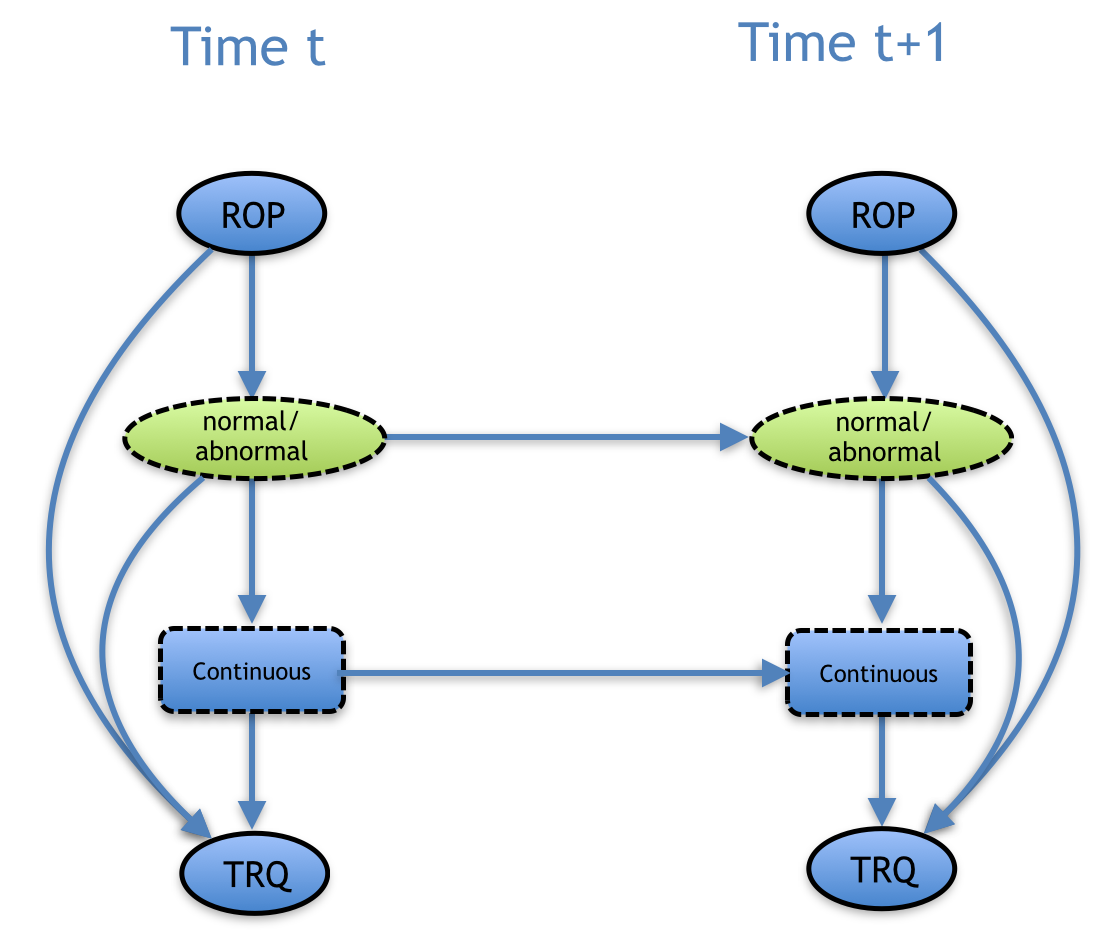
\includegraphics[scale=0.5]{./figures/VT_Scenario1} 
\caption{\label{Figure:VTScenario1} Input-output SKF structure used to detect abnormal TRQ states that cannot be explained by the observed ROP.}
\end{center}
\end{figure}

Further extensions to the model, where also other predictive variables are taken into account, will be considered at a later stage. The general model structure will, however, not be changed.

%-------------------------------------------------------------------------------------------------------------------------------------------------------------------
\subsubsection{Semi-automatic labelling}\label{SubSection:SemiAutomaticLabelling}
%-------------------------------------------------------------------------------------------------------------------------------------------------------------------

The main contribution from DrillEdge during operation is that it enables the driller to see in real time if the current situation is ``similar'' to previous situations that lead to undesired circumstances. If this is the case, remedial actions can be found to avoid undesired events. At the core of the analysis are historical examples of noteworthy episodes, ranging from clearly undesired events, for instance getting stuck, to more subtle indications of evolving problems, such as abnormal readings of hook-load. Verdande Technology has already extensive datasets (made available to the project from its beginning), where such episodes are identified. 
However, the definitions of the episodes are not always crisp, and domain experts can at times disagree about what is happening at a certain time. 
This can potentially lead to inconsistencies in the dataset, complicating both the automatic learning of models as well as the comparison with previous situations. 
Additionally, it can confuse the driller to be presented with information that he/she does not relate to or agree with.

Manually labelling new data sequences, or adapting the existing labelling to new definitions, can be a very time-consuming activity, and Verdande Technology therefore want to start looking into techniques for semi-automatic labelling.
This process is initiated by the system being fed with unlabelled data streams from typical drilling conditions. The system should adapt to this data, and recognise what is ``normal'', both with respect to auto-correlations of each variable over time, as well as the intricate relationships between variables. Simultaneously, sub-sequences that do not fit well with the normal data should be marked as ``abnormal''.
The abnormal sub-sequences can thereafter be examined more closely by drilling experts. It is desired that the process should be able to take back information from this examination, and update the reasoning if the sequences marked as abnormal were not correctly labelled. The benefit of the automatic tagging is that more time can be spent on scrutinizing the ``interesting'' parts of the drilling logs, and less time on the ``normal'' parts. 
This implies the potential for further reduction in non-productive time. Specifically, the goal is to provide a ``normality'' score for historical logs to facilitate semi-automatic detection of abnormal situations. The calculations should be efficient enough to run in real time if so desired.

Drilling is performed in phases, where different activities are conducted in sequence. For instance, one can only drill the well (increase the length of the well-bore) after having transported the drill-bit to the bottom of the well (that is, performed a ``tripping-in'' activity). Similarly, a long drilling sequence is split up into smaller sequences, where each subsequence is initiated by a ``connection'' activity, where the length of the drill-string is increased.
The division of the drilling log into subsequences containing only a single activity is done automatically by Verdande Technology's Drill Edge system. 
Therefore, the AMIDST system will be fed sequences where a single activity is conducted. 
The behaviour during each of these sequences  is fairly consistent if the process runs smoothly, and the relationships between variables can be established (e.g., the amount of mud transported into the drill-string will, after stabilization, can be a strong indicative of the amount of mud coming out after circulating through the well string). 

Some of the variables in the data set are used to monitor quantities that are set externally by the drilling crew (examples include ``weight-on-bit'', ``rotations-per-minute'' and ``mud-flow-in''). Other variables, like ``torque'', ``rate-of-penetration'' and ``pressure'' can be understood as (possibly delayed) responses to the input from the geology. 

As said above, the real-time parameters in drilling can to some extent be divided into control and response variables, where the great unknown is the physical properties of the formation that is penetrated.  The cause $\rightarrow$ response relationships are mostly unknown, but some qualitative understanding exists. 

The model we propose for this task is similar to the one proposed in the previous application scenario . It is detailed in Figure \ref{Figure:VTScenario2} and has again an \emph{input-ouput} Kalman filter structure with observed control variables on top and the observed response variables down. The main difference now is that the discrete variable is not temporally linked and does not try to capture any ``physical'' property of the process. This discrete variable is simply included to improve the modelling capacity over the observed response variables because it allows now to model mixture of Gaussians for these variables. 

As commented above, this input-output SKF  will be used to model the ``normal behaviour'' of the well. The ``abnormal behaviour'' will be detected using the following protocol.  The normality-index for each observation at time $t$, denoted by ${\bm x}_t$, given the observations up until $t$, denoted by ${\bm x}_{1:t-1}$, will be calculated as the log conditional likelihood, $\ell_t := \log p\left({\bm x}_t|{\bm x}_{1:t-1}\right)$, where $p$ is the probability distribution induced by our input-output SKF. By monitoring $\ell_t$ over time, significant departures from its ``typical behaviour'' will be noted, and marked as potential irregularities.


\begin{figure}[ht!]
\begin{center}
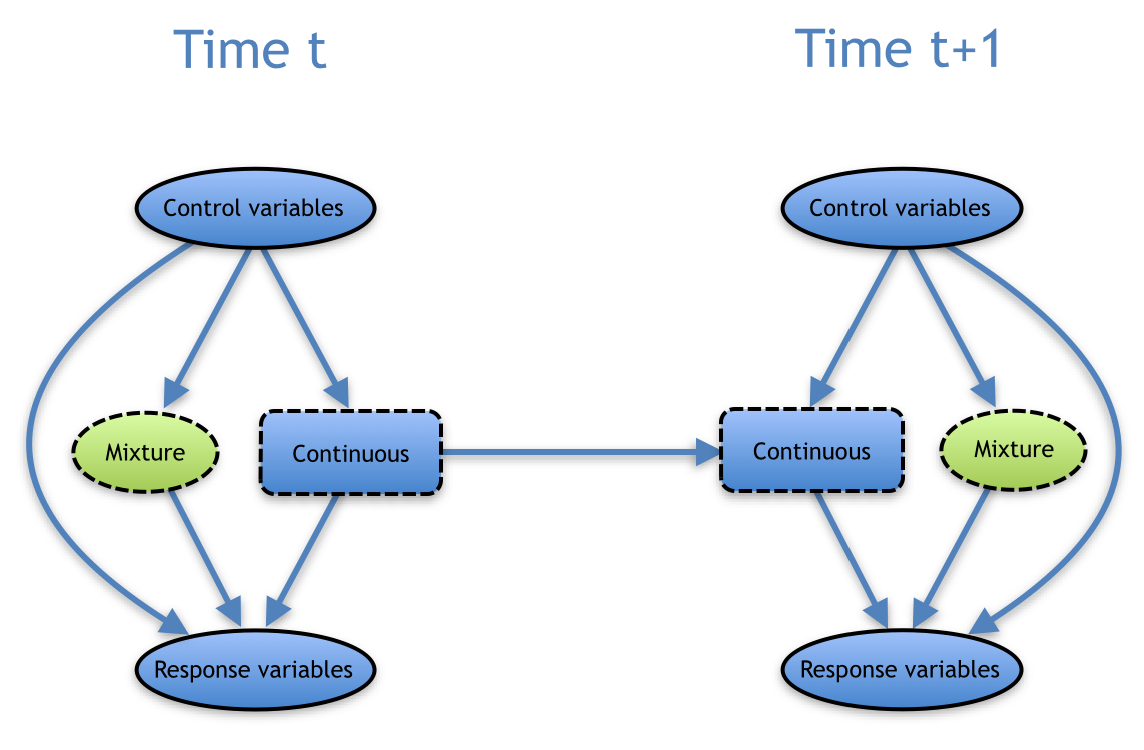
\includegraphics[scale=0.5]{./figures/VT_Scenario2} 
\caption{\label{Figure:VTScenario2}  Input-output Kalman filter with Gaussian mixtures at the leaves used for semi-automatic labelling.}
\end{center}
\end{figure}

\textcolor{red}{\bf Do we need to show the structure of the analysis for the $\ell_t$-terms?}

%-------------------------------------------------------------------------------------------------------------------------------------------------------------------
\subsubsection{Automatic formation detection}\label{SubSection:DetectionFormation}
%-------------------------------------------------------------------------------------------------------------------------------------------------------------------

In many drilling operations, a precise recognition of a formation change can be vital for cost savings. 
For instance, it is important to cement the casing in the correct formation to manage the formation pressures, as well as correctly identifying the top and the bottom of an oil reservoir. 
Additionally, accurate knowledge of the formation allows the drilling crew to optimise drilling parameters and better diagnose the condition of the bit. 
Knowing the formation is also an important input in how to deal with symptoms such as improper hole-cleaning, hole-instability and vibration issues. 
A proper formation detection is therefore an important piece in the puzzle for reducing the overall non-productive time.

Before the well is drilled, a chart with the expected formation tops is available from the well plan. The chart is based on seismic data and drilling data from neighbouring wells and contains the best guesses on which depths the various formation tops are located. Since it is uncertain where the formation tops are, an uncertainty interval is associated with every formation top. This is called the lithology chart. 

In practice, the prediction of the formation tops is refined by a human, who interprets  {\em measurement while drilling} (MWD) data and aligns this with the lithology chart as the well is being drilled (see Figure \ref{lithology}).

\begin{figure}[ht!]
\begin{center}
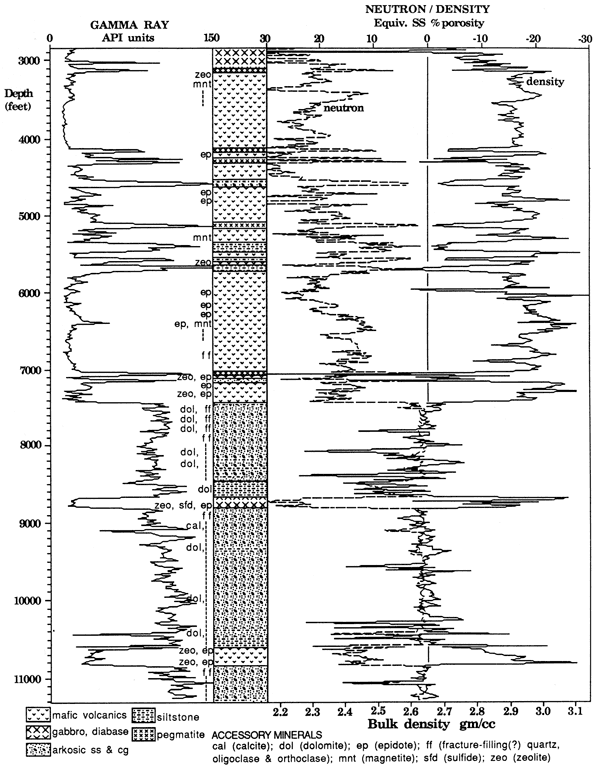
\includegraphics [keepaspectratio,width = 10.7cm] {figures/VT_lithologyGamma.png}
\caption{Lithology data shown together with petrophysical measurements such as gamma radiation and neutron/density.}
\label{lithology}
\end{center}
\end{figure}

The MWD data measures petrophysical properties of the rock such as gamma radiation, sonic speed and electrical resistivity. 
Often, shifts in these graphs happen when the formation is changing. We will therefore formulate the formation detection problem as change-point detection in a multivariate data stream. 
Indications of change-points (shifts) are to be compared with the prior belief to specifically locate the changes. The model described below is built to capture \textit{instantaneous} changes in formation, and is not made to capture gradual changes. 

The prior information, giving the expected locations (depths, in meters) of formation change, together with a degree of certainty (in terms of a standard deviation) is the point of departure for this model. Let us assume that the drilling crew, a priori, expects  to see $N$ changes in formation. 
This information may be erroneous, as any number of additional formation-changes (that were not expected in advance) may also occur in the ground, e.g., formation of sandstone can be a priori expected for 100 meters, later realizing that this sediment was split into two by a small layer of shale.
The observation data is encoded wrt.\ \textit{time}, but will be used with an encoding wrt.\ \textit{depth} in this application to have it aligned with the prior information at hand. The data may not necessarily be equally spaced (e.g., two neighbouring observations may be separated by half a foot, while the two next are separated by only a tenth of a foot). 
 
In this case, we think in terms of an IOHMM (see Section \ref{SubSubSection:HMMs}), in which the latent variables will have a predefined structure (see Figure \ref{Figure:VTScenario3}):

\begin{figure}[ht!]
\begin{center}
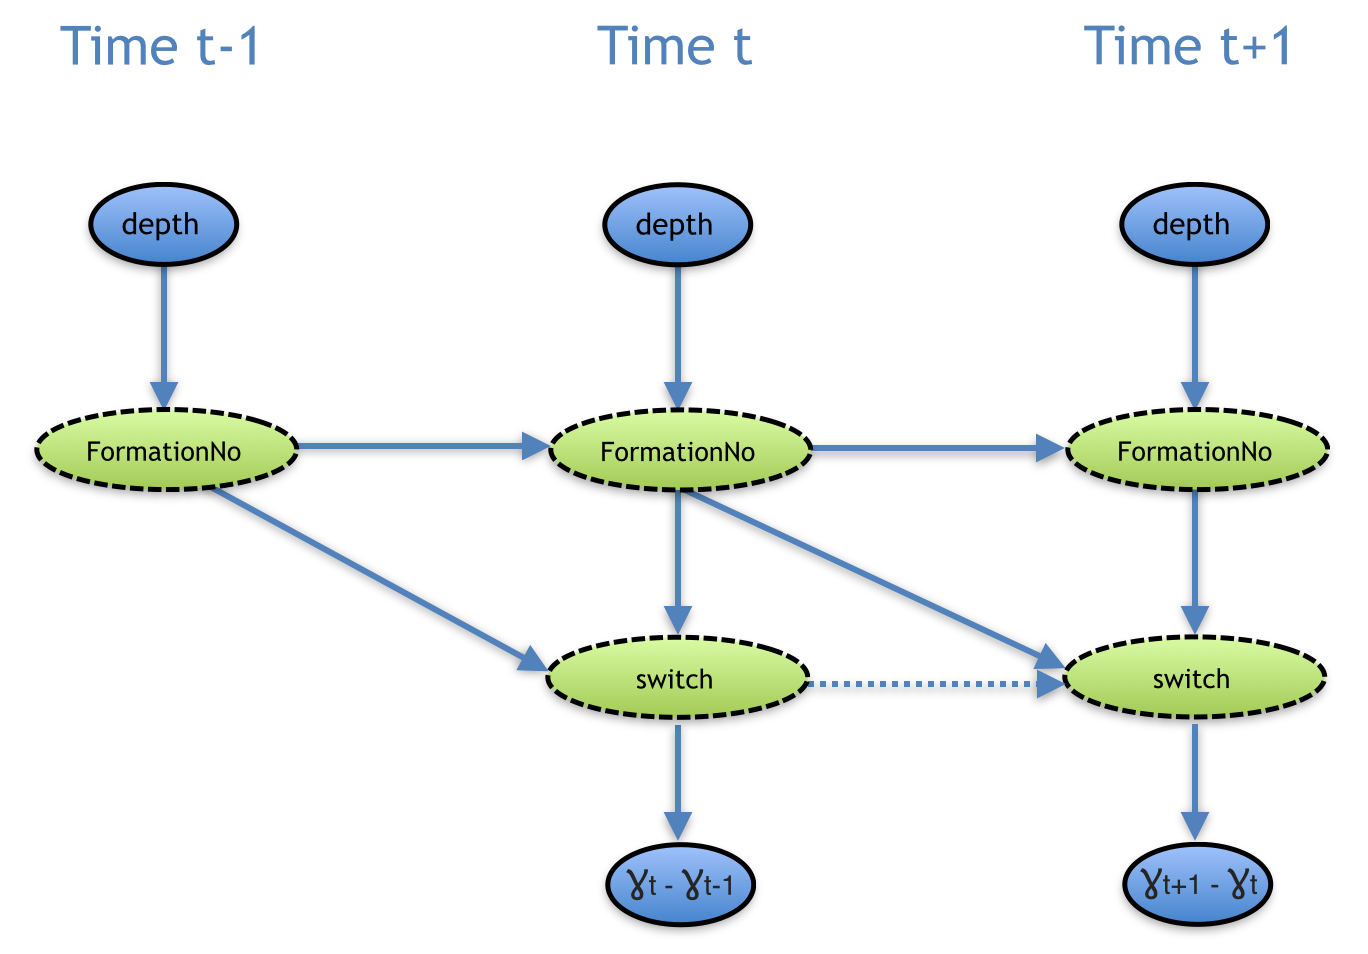
\includegraphics[scale=0.5]{./figures/VT_Scenario3} 
\caption{\label{Figure:VTScenario3} Input-output HMM used for formation detection. The output observed variables $\gamma_t-\gamma_{t-1}$ represent the differences of consecutive gamma ray observations.}
\end{center}
\end{figure}

\begin{itemize}

\item The input variable at time $t$, Depth$_t$, is the depth of the bit at that time.

\item The next chain of variables are \textit{counting-variables}, denoted by  FormationNo$_t$. The variable has two parents: Depth$_t$ and FormationNo$_{t-1}$. 
The probability that the counting variable is incremented at time $t$ conditioned on the parent configuration is calculated by combining information from the prior information with the parents' configuration. Logistic or probit functions can  be imagined, but must be compared to the actual domain knowledge to give a feasible representation.
Note that the model structure, with  a continuous parent having a discrete child does not entail computational difficulties in this case: The parent is always observed, and the calculation of the conditional probability table (encoding the transfer function) can thus be done externally. The model thus capture a non-stationary process by conditioning the transition distribution to the observed control variables. 

\item Shift$_t$  generates a  chain of variables used for determining when   a formation-change actually occurs. It has two parents, namely  FormationNo$_{t-1}$ and  FormationNo$_t$. 
The variable is discrete, and has four states: ``No -- As accounted for in the prior'', ``No -- But expected in prior'', ``Yes -- As accounted for in the prior'', and ``Yes -- But not expected in prior''. 
To this end, FormationNo$_t$ only changes when expected by the prior information, while Shift$_t$ can use the data to refine these assessments. If $\mbox{FormationNo}_{t}= \mbox{FormationNo}_{t-1}$, Shift$_t$ is in the state 
 ``No -- As accounted for in the prior'' with probability $1-\epsilon$ and in state ``Yes -- But not expected in prior'' with probability $\epsilon$. If $\mbox{FormationNo}_{ t}=\mbox{FormationNo}_{t-1}+1$, Shift$_t$ takes the state 
``Yes -- As accounted for in the prior'' with probability $1-\delta$ and ``No -- But expected in prior'' with probability $\delta$. $\epsilon$ and $\delta$ are parameters to be determined through expert knowledge or learned from data.

\item Finally, the observed variables at time $t$ only have  Switch$_t$ as parent. We will not use the actual observed sensor reading as the observed variable (``output-variable'' in the input-output model). Rather, the differences are considered, e.g., GammaRay$_t$ - GammaRay$_{t-1}$ will be used to represent the gamma ray measurement at time $t$. These variables will, given that Switch$_t$ is in the ``No''-states, vary around zero. The variable will be significantly different from zero if the parent is in any of the ``Yes''-states.  It is clear from Figure \ref{lithology} that most formation changes are seen as clear shifts in the gamma ray data.
\end{itemize}

At the time of inference, we condition on the total number of switches, and calculate (using forward-backward) the posterior distribution of the locations. Similarly, we will also calculate the most probable explanation, that is, the most probable configuration of switches given the total number of events.

%-------------------------------------------------------------------------------------------------------------------------------------------------------------------
\subsubsection{Discussion and future models}
%-------------------------------------------------------------------------------------------------------------------------------------------------------------------

The models presented above, describe a first attempt to address the tasks involved in the Verdande problem domain. A first critical question to the model for erratic torque is that the model assumes the observations from a tach of data without erratic torque to follow a Gaussian distribution. Secondly, the assumption that erratic torque is manifested through an additive high-correlated Gaussian noise must be verified as well. A natural first step is to experiment with the model on synthetic data simulated from relevant (but non-Gaussian) distributions to quantify its robustness wrt.\ these assumptions. Secondly, a critical investigation into the results obtained when running on real data will be conducted, potentially leading to  more expressive models having to be utilized. 

%%%%%%%%%%%%%%%%%%%

The semi-automatic labelling model is so far made using a general-purpose model structure, that does not encode a priori domain knowledge. As more domain knowledge is uncovered (see the upcoming Deliverable 7.1), we will consider to make structural changes accordingly. 

%%%%%%%%%%%%%%%

The model for formation detection assumes that changes in the logged data happen instantaneously. Instantaneous ``jumps'' are observed for, e.g., the gamma ray measurement, but may not be equally valid for other variables, like resistivity. If required, a richer model (albeit contained inside the class of input-output models) may have to be addressed, where the observations themselves (and not their time differences) are utilized. Furthermore, we have again  assumed that the difference in an variable between two observations follows a Gaussian distribution with fixed variance. The assumption must be better validated with other data sets and amended if required.





